% -------------------------------------------------
% How Green?
% Human Computer Interaction (H) Coursework
%
% "Your report should be a maximum of 10 pages. It should include information about your design concept (and why it is interesting and valuable), your design process, the stages of implementation you went through, and the evaluation(s) you did of the design(s). You should also reflect on the system you designed and show how it might be improved in the future."
%

\documentclass[a4,10pt,twocolumn]{article}

%==============================================================================
%% Packages and Command Setting

\usepackage[margin=1.5cm]{geometry}
\usepackage{svg}
\usepackage{minted}
\usepackage{hyperref}
\usepackage{titlesec}
\usepackage{graphicx}
\usepackage{biblatex}

\definecolor{bg}{rgb}{0.95,0.95,0.95}

\immediate\write18{[[ ! -f "assets/logo-black.svg" ]] && sed 's/00D98F/1c1c1c/' assets/logo.svg >assets/logo-black.svg}

\addbibresource{references.bib}

\setlength{\parindent}{0pt}
% \titlespacing\section{0pt}{8pt plus 4pt minus 2pt}{0pt plus 2pt minus 2pt}
% \titlespacing\subsection{0pt}{8pt plus 4pt minus 2pt}{0pt plus 2pt minus 2pt}
% \titlespacing\subsubsection{0pt}{8pt plus 4pt minus 2pt}{0pt plus 2pt minus 2pt}

\title{%
    
\includegraphics{assets/CompSci_mono}\\[\bigskipamount]
    {\Large Human Computer Interaction (H) Coursework \par}
    \vskip 1em%
    \includesvg[width=200pt]{assets/logo-black.svg}\par
    \vskip 1em%
    {\LARGE How Green? \par}
    \large
}

\author{%
    Anna Berry\\
    Hector Jones\\
    Inesh Bose\\
    Marc Auf der Heyde\\
    Stephen Connolly
}

\date{}

\begin{document}

\onecolumn
\maketitle
\vfill

\noindent{\bfseries Abstract}\par
\noindent In the following report, we seek to outline the underlying development and evaluation process, leading to the creation of our sustainability browser extension, How Green. This report will examine each iteration of prototyping, and look at the accompanying usability evaluations conducted at each iteration. \bigskip

\noindent{\bfseries Declaration of Originality}\par
\noindent We confirm that this assignment is our own work and have
\begin{itemize}
    \itemsep0em
    \item Read and understood the University of Glasgow Statement on Plagiarism.
    \item Clearly referenced, in both the text and the bibliography or references, all sources used in the work.
    \item Fully referenced and used inverted commas for all text quoted from books, journals, web etc.
    \item Not made use of the work of any other student(s) past or present without acknowledgement, or sought or used the services of any professional agencies to produce this work.
\end{itemize}
\noindent In addition, we understand that any false claim in respect of this work will result in disciplinary action in accordance with University regulations. \bigskip

\noindent{\bfseries Education Use Consent}\par
\noindent We hereby give our permission for this project to be shown to other
University of Glasgow students and to be distributed in an electronic
format.

%\newpage
\twocolumn

%==============================================================================
%% Understanding Requirements

\section*{Understanding Requirements}
% All of these subsections are not relevant but can use some
In this section, we will examine the process underlying the development of How Green?, our browser extension, which we built to help online shoppers find more sustainable food products to purchase. We will introduce our App Definition Statement, reference some existing solutions that acted as the basis for our initial idea and discuss the process used to identify initial core requirements.

\subsection*{App Definition Statement}

A browser extension to make finding sustainable food products online, simple. 

\subsection*{Existing Solutions}
We decided to focus on sustainability, specifically the sustainability of food products. We began by looking into existing websites and applications to identify what was currently available in the market and to make sure that our idea would be unique.

There are many existing websites that focus on sustainability. For example, Ethical Consumer \cite{EthicalConsumer} provides users with tools and resources to make better shopping choices, providing information on companies and products. The 2030 Calculator \cite{2030} is a tool that can calculate the carbon footprint of a product.

Food is an area of sustainable shopping that is focused on by many websites. SU-EATABLE LIFE \cite{SU-EATABLE} is a website financed by the EU LIFE program that aims to reduce the environmental impact of food choices through engaging with and informing EU citizens of their foods impact. The application evocco \cite{evocco} also focuses on the sustainability of food allowing users to scan receipts to keep track of the climate impact and carbon footprint of their food shopping. Specific online stores also exist for carrying out ethical food shopping. La Fourche \cite{LaFourche} offers consumers organic food in one place while helping shoppers save money. Finch \cite{Finch} is a company developing a browser extension that will provide insights into products sustainability using custom technology. The browser extension is currently still in development. 

\subsection*{Initial Core Requirements}
The team discussed initial ideas based on our market research into existing products and decided on developing a browser extension as this was something currently missing from the market. The core requirements for this project were gathered within the development group after discussions during the first project meeting. The core requirements included:

\begin{enumerate}
    \item The Browser Extension should allow users to see how sustainable a product is as a score.
    \item The Browser Extension should be easy to use, intuitive and unobtrusive when shopping.
    \item The Browser Extension should link to a website where more information can be gathered.
    \item The Browser Extension should use Information visualisation to display information on products.
    \item The Information visualisations should allow for active engagement made available through our product.
    \item A Minimum Viable Product (MVP) should be produced.
\end{enumerate}

From these core requirements, we started our concept generation, a process in which we took our initial starting idea and refined it over multiple iterations to help guide us in the development of our MVP.

%==============================================================================
%% Concept Generation

\section*{Concept Generation}
After discussing initial ideas of sustainable projects to pursue, the group discussed and evaluated the benefits of each idea, and after some deliberation agreed to develop what would go on to be called How Green? 

Our process for concept generation was through group discussions, in which we came up with viable ideas and decided on which ones the group liked the most and and fit our core requirements. One idea discussed by the group was a browser extension that would show how sustainable a product is that a user was trying to buy. The sustainability would be based on a score provided by the browser extension. An alternative idea explored was to develop a multi-user game experience educating users on their active screen usage each day and exposing users to the ad market. This idea was not pursued given that it failed to meet our core requirement of sustainability.

From our concept generation we decided on a sustainability Browser Extension that would focus on users' online shopping experience, given the apparent gap in the market as well as personal interests in developing something related to climate change. To meet the core requirements, we decided products would be given a grade A-D and a percentage correlated to that grade - the higher the grade the more sustainable a product is. The grading scale is easy and familiar for users to understand. We decided that the browser extension would link to a website where further information explaining how the grade was calculated could be displayed, alongside interactive graphs to help explore this information visually.

We also went through a process of name generation to choose a name that would represent what the browser extension and website would do. Brainstormed names included Save the Trees, GreenerAlts, Greenazon and finally, How Green?. We decided on the name How Green?, given green is commonly used as a synonym for how sustainable something is and the question mark representing a user's query regarding how sustainable a product is.

Once the concept was finalised, we decided to begin prototyping our Browser Extension to finalise our ideas and make sure we met our core requirements.

%==============================================================================is
%% Initial Prototyping

\section*{Initial Prototyping}
In this section, we will discuss the initial prototyping process that led to the final implementation of our MVP. Specifically, we will provide details of the early product prototypes developed and the evaluation methods applied to these prototypes. From these evaluations, we will present the logical refinements that followed that led to the final implementation of our MVP. After finalizing our initial ideas, we decided to begin with an immediate low-level user evaluation. 

\subsection*{Paper Prototype and Focus Group}
A paper prototype incorporating the core elements of our initial idea was developed to be used in a focus group usability evaluation. The paper prototype, which can be seen in Figure 1, was divided into three sections displaying three different system states we wanted the product to support.
\begin{itemize}
    \item \textbf{Idle mode:} the browser extension sits idly in the browser toolbar, waiting for an action from the user.
    \item\textbf{Cost calculated mode:} the browser extension shows a score in the form of a percentage or grade for the current product a user is visiting. On the same view are two buttons, one that links to an extended report of the score and one that links to produce alternatives for the relevant product.
    \item\textbf{Extended report mode:} the browser extension opens a separate tab, displaying a detailed information visualization regarding the calculated sustainability score for the currently viewed product. The information visualizations are interactive and can be used to help make smart decisions when evaluating and choosing products based on sustainability.
\end{itemize}

\begin{figure}[h]
    \centering
    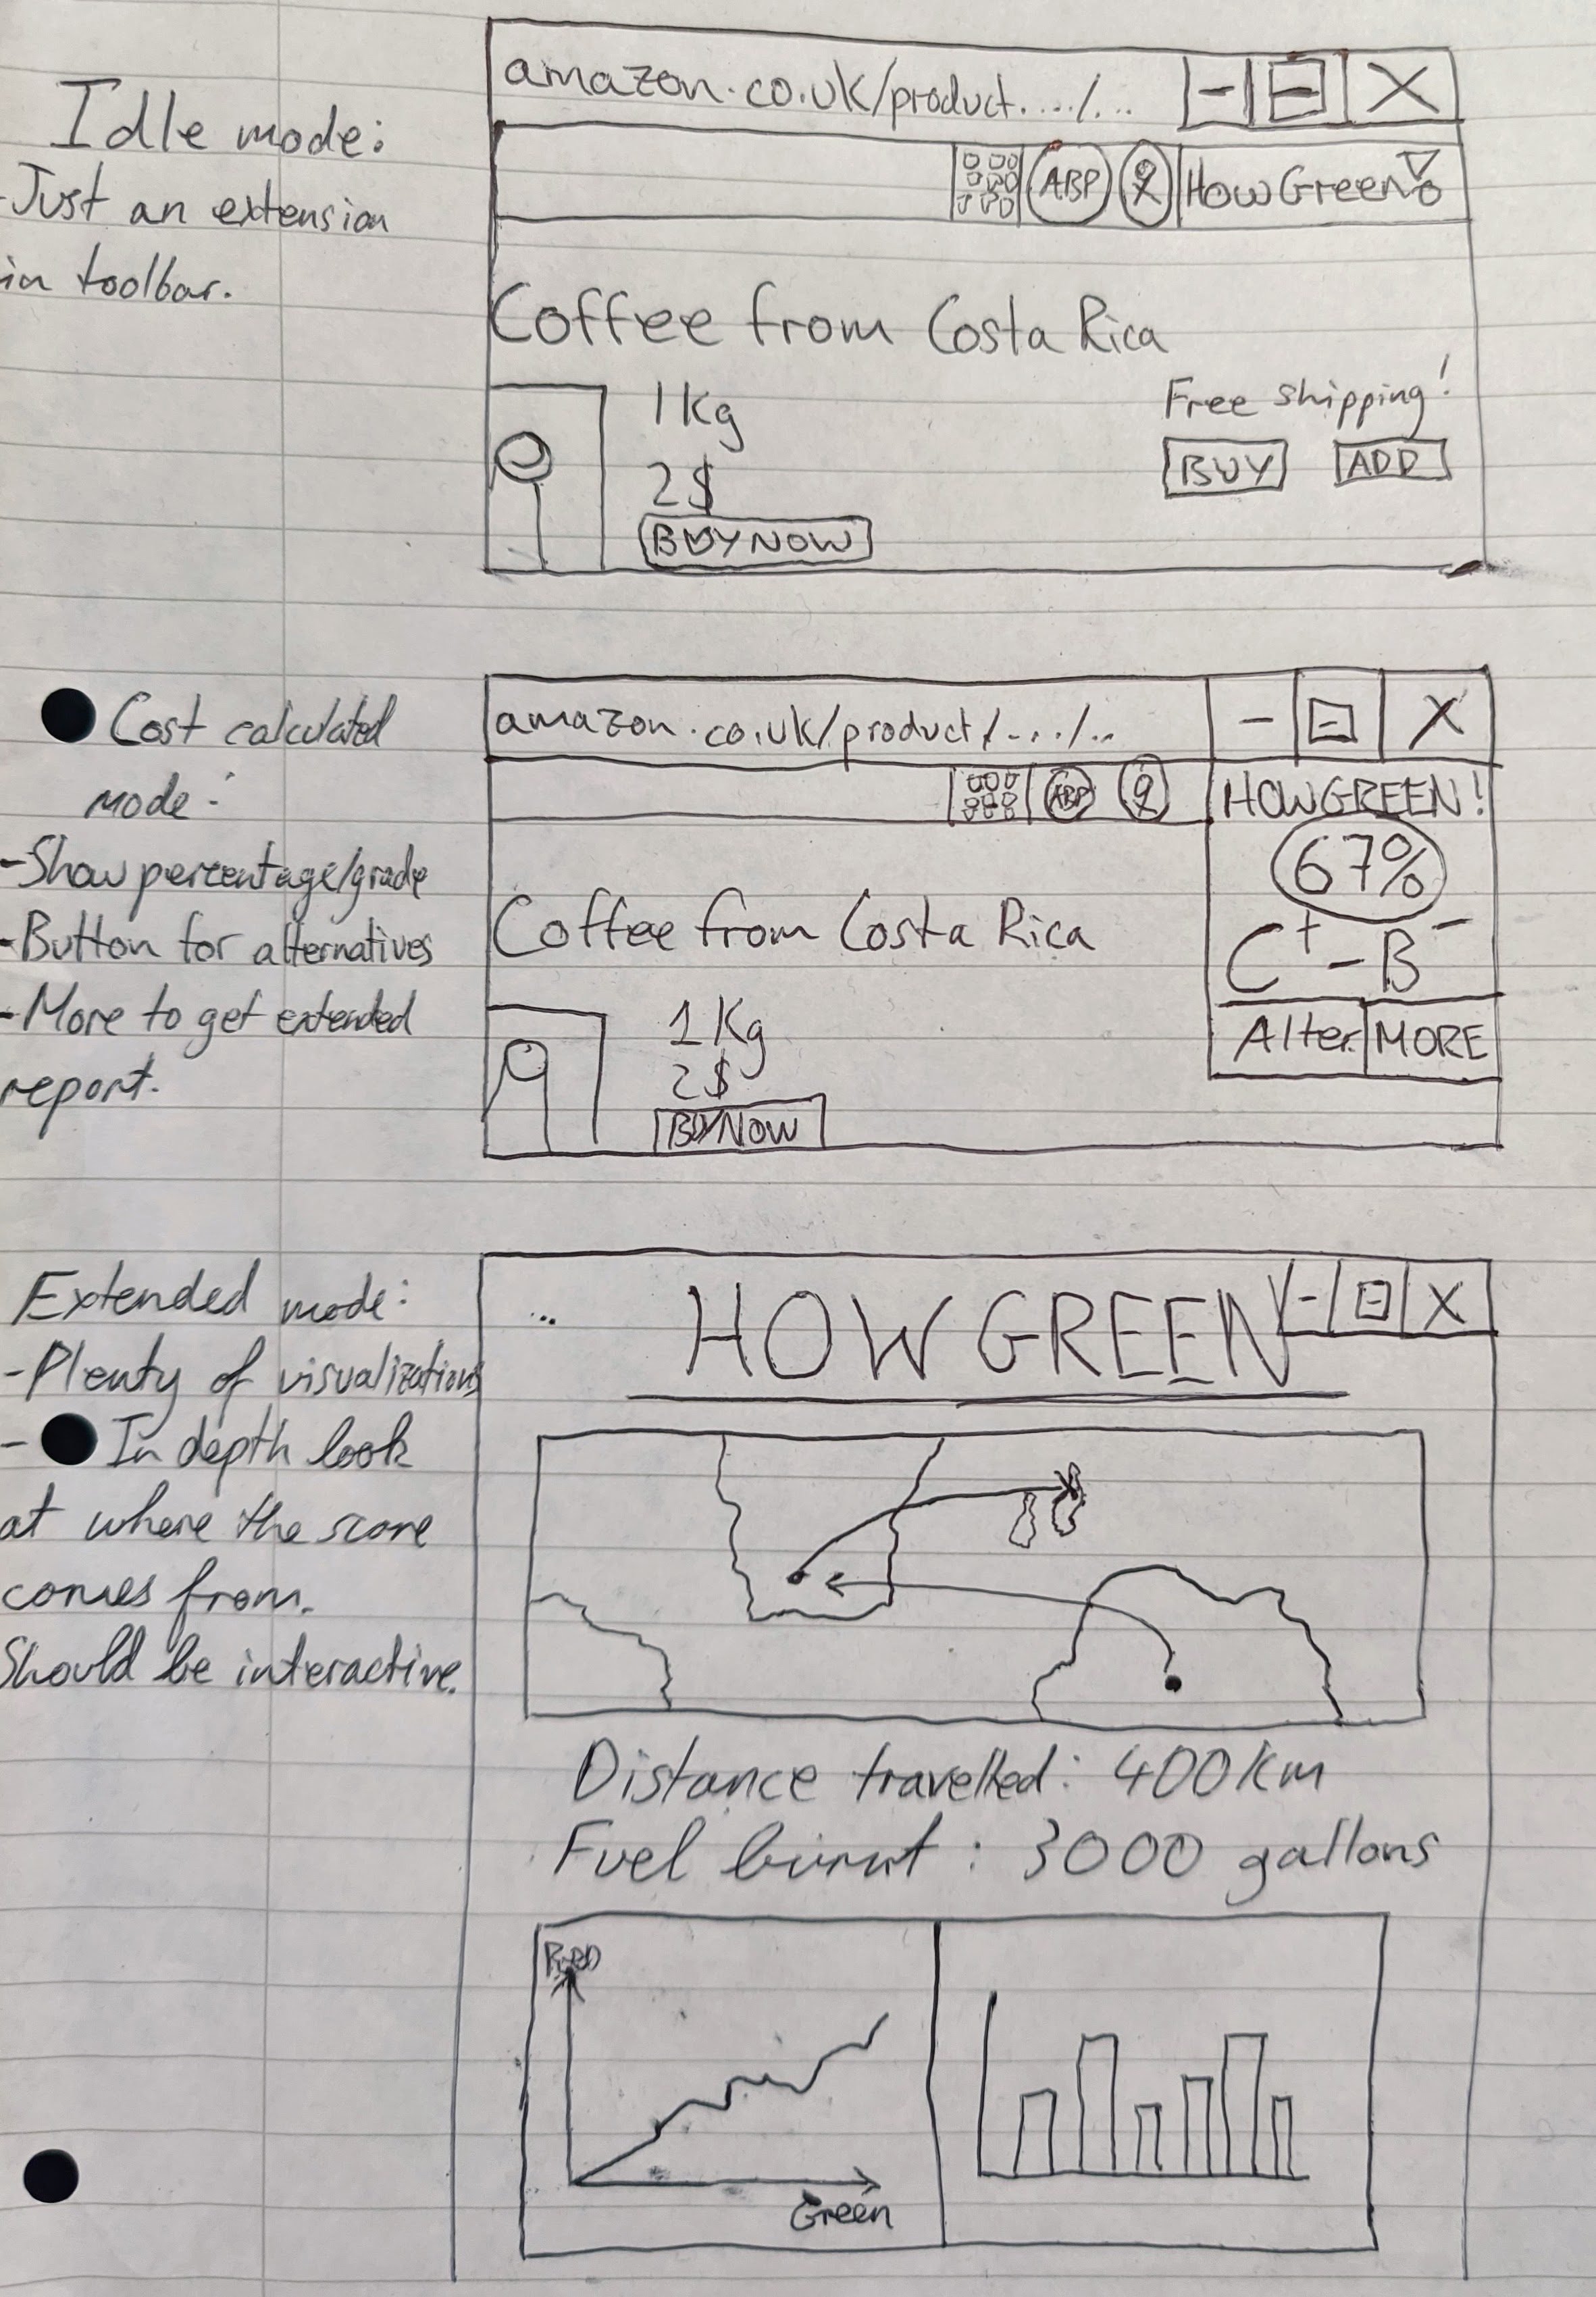
\includegraphics[width=0.9\columnwidth]{assets/prototype/paper_prototype.jpg}
    \caption{Paper Prototype sketches}
\end{figure}

A focus group was than conducted using the developed paper prototype as a visual aid to support the focus group discussion. The focus group was made up of 3 female participants, aged 21-23. The Focus Group was split into three distinct discussion parts and the results of these discussions were:
\begin{itemize}
    \item \textbf{Climate change awareness:} In this section of the focus group, we tried to gain an understanding of how aware the participants in the group were of climate change, with emphasis on aspects like their carbon footprint and energy conservation. Generally, all members of the group were aware of climate change and how bad their carbon footprint might be. They agreed that they do not actively try to reduce their carbon footprint, however if the opportunity is made available, they do. 

    \par All members also agreed that climate change was something that needed to be tackled on an individual basis and mentioned that they all had some experience in making individual consumer decisions influenced by their climate change awareness. An example of such a decision was given, referring to choosing between multiple crisp packet options, where one participant highlighted the influence of individual packaging on their consumption of crisps. 

    \item \textbf{Shopping experience and climate change awareness:} In this section of the focus group, we wanted to understand more clearly how users' climate change awareness might contribute to their overall shopping experience. We investigated brand awareness participants might practice when selecting food products, as well as the degree to which participants might be influenced by such information. We provided examples of products from brands known to be particularly sustainable such as Scottish Spring, and brands known to be particularly non-sustainable such as Nestle.

    \par All participants agreed that they were aware of different brands of products having differing effects on the environment. One participant noted that although aware of the effects of many brands on the environment, they were also aware of the efforts made by brands to separate their image and reputation from their effects on the environment. This made the participant skeptical that they could accurately distinguish between two different brands' effects on the environment. 

    \par All participants agreed that knowing the effect of a brand on the environment would influence their decision to purchase that brand, and extended this to suggest that they would seek product alternatives if they were made aware about a particular product's negative impact on the environment. 

    \par Perhaps most interestingly from this section, we also investigated what category of products consumers would care most about in terms of finding more sustainable options. Though all participants agreed that when online shopping, food was the least purchased item, they did say that food and groceries would be of most interest to them in terms of sustainability. Clothing would be the next best category to service. This result of the focus group would be essential in helping guide the development of our final MVP. 

    \item \textbf{Prototype specific questions:} In this section, we presented the participants of the Focus Group with the paper prototype we had developed and asked them specific questions relating to the prototype. This section was the driving factor behind the refinements made from our prototype and implemented in our higher-level interactive Figma prototype.

    When asked if they would use a browser extension to aid them in finding more sustainable products, all participants responded that dependent on the design of the extension, they would all use the extension. Two of the three participants liked the idea presented in the prototype to Honey \cite{Honey}, a browser extension that finds discount codes to be applied on checkout pages of online shops. On this note, they remarked that the Honey user experience was enjoyable, given that it was there but non-intrusive; it can be used when the user wants to use it, but not at the cost of annoying the user. This highlighted an important trade-off in the design of such a browser extension. Specifically in our case, we were intending to prompt users to some degree given that participants said they were often too lazy to find alternative, more sustainable products themselves, but realized that it could not be too much as to impact the overall user experience. 

    Before discussing the specifics of the paper prototype, participants had some additional information as to what would increase the likelihood of using the proposed system. One such feature, would be the ability to find local alternatives when shopping online, to support local producers more directly. If the project was being continued, this would have been made a must-have-feature of the end-product. Due to time constraints however, this was excluded from the final design. 

    Participants were unable to suggest a better alternative to a browser extension that would aid in their search for more sustainable product alternatives. In fact, they reiterated why a browser extension would be most suitable, referring again to Honey as an example. When shown examples of how a product rating should be displayed, referencing their desire to have a quick estimate for quick decision making, participants agreed that a traffic light system (green = good, yellow = OK, red = bad), would be suitable for quick reporting on a product's sustainability. A percentage and/or letter grade would also be seen as suitable, provided there was sufficient information to clarify what a letter grade or percentage meant in terms of sustainability. Participants also expressed their desire for a warning system, to indicate when users might be about to purchase a particularly unsustainable product.

    When asked how they would like to be shown alternative products, participants responded that they would like some kind of consistency with the website they were browsing, perhaps showing the alternatives as a shopping list or similar structure. To avoid confusion, participants mentioned that the alternatives should be available to view on a dedicated page, like the extended report in the prototype. One participant also expressed their desire to categorize alternative products according to filters such as popularity or price. 

    Lastly, the participants thought of some of the metrics that would be important to them in the calculation of a sustainability score and discussed some mediums for displaying this information visually in an intuitive and interactive way. Transport in production, sourcing of raw materials, sourcing of labour force, amount of energy used in production, product's local availability, price and company profits were all metrics the participants would like to be included in the calculation of the sustainability score.
\end{itemize}

The thoughts of the focus group was used as the primary motivator for the refinements made from the paper prototype to the interactive Figma Prototype. Many of the results of the Focus Group would become some of the core features of our MVP, specifically the balance between prompting users to make good decisions without being too intrusive.

After having processed the results of the focus group, development of the first interactive prototype, a Figma prototype, begun, with the aim of conducting a usability evaluation using this refined prototype to prepare in the development of our MVP.

\subsubsection*{Interactive Figma Prototype and think-aloud usability study}

We decided as a group to use Figma for implementing a prototype of How Green? as it is easy to use with a short learning curve, allows us to go between pages and all group members can work on the prototype simultaneously. To being, we took screenshots of the Tesco page with a selection of products and developed a basic extension page to show the calculated score of the product as well as a link to alternatives and details of how the score has been calculated.
\begin{figure}[h]
    \centering
    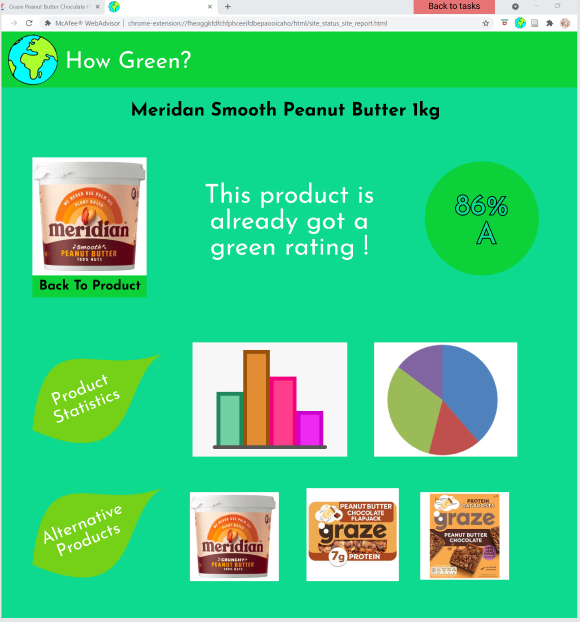
\includegraphics[width=0.9\columnwidth]{assets/prototype/figma.PNG}
    \caption{More Information About A Product Page}
\end{figure}

\begin{figure}[h]
    \centering
    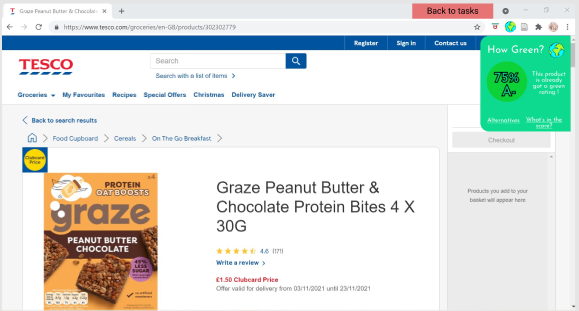
\includegraphics[width=0.9\columnwidth]{assets/prototype/figma_extension.PNG}
    \caption{Browser Extension}
\end{figure}

The features supported on the Figma prototype were:
\begin{itemize}
    \item \textbf{View Score}: Show the calculated score of the product.
    \item\textbf{View Alternative Products}: Show alternative products with their corresponding score and colour.
    \item\textbf{Home Page}: Introduce the user to How Green? and gives them an overview of what we believe in.
    \item\textbf{Browse Tesco}: Allow the user to browse the Tesco website so they can view any product they want and see the score.
    \item\textbf{View Graphs}: Show the user a basic graph to give an idea of what the final product will look like.
    \item\textbf{More Information}: Show the user a more in-depth look into what is used to calculate the score, linking to alternative products and product statistics.
\end{itemize}

After we had a finished first version of the prototype, we conducted a think-aloud study with 15 anonymous participants from a sample population. This allowed us to gather unbiased data that we could then analyse. We wanted the participants to have a full walk through of the prototype so made sure to cover all bases with the questions.     

\subsection*{Prototype evaluation}
% Summarize the results of the Figma think-aloud and survey results
The participants were asked to perform a series of tasks to evaluate the usability of our Figma prototype. The tasks are as follows:

\begin{enumerate}
    \item Visit the browser extension homepage (this can be accessed by clicking the icon in the top right).
    \item Visit Tesco peanut butter search selection.
    \item Select a product you want to view.
    \item Check the score provided by the browser extension for that particular product. 
    \item Show further information from the browser extension.
    \item Find alternatives for the current product.
    \item Show an extended report of the calculated score for that product.
    \item Interact with the graphs provided by the browser extension.
\end{enumerate}

A brief summary of our think-aloud evaluation results, specifically which tasks were of particular difficulty in terms of completion, and overall comprehension of the system are as follows:

\begin{itemize}
    \item The most common frustration among participants was not being able to go directly back to the main extension overview page for a product from either the alternatives or the graphs pages, due to the prototype not having back buttons that would allow this.
    \item There was general confusion with the task for showing an 'extended report' for the product, as it was unclear from the browser extension that the 'What's in the Score' button meant this.
    \item Many participants had issues going to the product pages of alternatives for a given product. Since the button 'Go to Product Site' did not consistently work across all the pages, participants had to click on the alternative product's photo instead.
    \item On the alternatives page, participants mentioned displaying the current product score to be compared to the list of alternatives' scores would be useful for comparison.
    \item The scores presented, the grades and the percentages, resulted in confusion among participants, specifically what the scores meant and what values were used in calculating them.
    \item On the 'What's in the Score' page, it was suggested by some participants to not include a list of the alternatives and a list of graphs as there were already buttons redirecting the user to pages dedicated to these.
    \item The extension immediately popping up as soon as a participant landed on a product page was generally described as distracting. Preferably the extension would remain in the top right tool bar and only expand upon being clicked on.
    \item With regards to the visual design and aesthetics of the Figma prototype, participants mentioned that many of the images and icons were too square-like and this was not visually pleasing. Additionally, the colour scheme of white and green was said to make it difficult to read and perhaps different shades of green should be considered to make it more legible.
    \item With regards to the graphs page, their meaning was very unclear due to lack of legends and labels describing what they were about.
    \item Some participants also mentioned that making it clear exactly which buttons were clickable would have facilitated the performance of the tasks overall.
\end{itemize}

After completion of the think-aloud evaluations, participants were asked to complete a survey regarding their experience of the prototype. The survey featured questions relating to each task in terms of difficulty, as well as general design questions.

\begin{itemize}
    \item The difficulty score provided by participants for most tasks was considerably low, this indicated that the prototype had adequate usability. However, there were mixed scores given for both tasks 6 and 8.
    \item Some participants found it difficult to find alternatives in task 6. This may have been due to the lack of functionality in the prototype allowing users to go back from either the graphs or alternatives pages to the extension overview.
    \item The difficulty in finding the graphs for task 8 agrees with a few of the results of the think-aloud usability evaluation. Participants mentioned not being able to click on the 'Product Statistics' button on the main extension overview page, which should intuitively lead to the page specifically for graphs as it does for alternatives. Instead, to interact with each graph participants had to click on each image, which was not made obvious.
    \item There were generally positive results from participants with regard to the extension not feeling too intrusive or annoying, with only a few scoring it mid-range. This correlated with the participants in the think-aloud evaluation commenting on the pop up extension being slightly distracting and too big. Most participants also scored the prototype as being intuitive to use and across the board gave the design of the prototype a high score.
\end{itemize}

\subsection*{Refined Prototyping}
% Summarize the improvements made from the Figma to our final design, should correspond to what was extracted from the evaluation!
From our results of the think-aloud evaluation as well as our survey results, we were able to extract vital refinements to be made to our prototype. These can be summarized as follows:

\begin{itemize}
    \item Alternatives displayed in the prototype were made sure to be ordered from best score to worst score.
    \item Products of the same brand were made sure to not have drastically different scores as this caused confusion among participants.
    \item On the alternatives page, every 'Go to Product site' button was fixed to be clickable and redirected to the alternative product's appropriate Tesco page.
    \item The pop-up when clicking on the browser extension was reduced in size in accordance with feedback about it being too large and distracting.
    \item A final refinement was ensuring that the How Green? logo in the browser toolbar would not redirect to the homepage but instead for any instance of the logo on the extension pages to redirect back to this homepage.   
\end{itemize}
\begin{figure}[h]
    \centering
    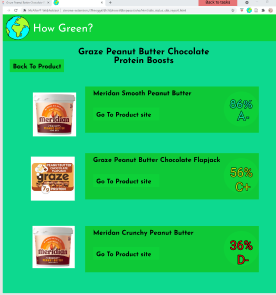
\includegraphics[width=0.75\columnwidth]{assets/prototype/pre_eval.PNG}
    \caption{Alternative Products Page pre Evaluation}
\end{figure}
\begin{figure}[h]
    \centering
    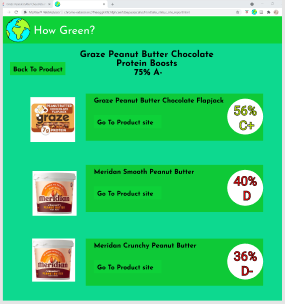
\includegraphics[width=0.75\columnwidth]{assets/prototype/post_eval.PNG}
    \caption{Alternative Products Page post Evaluation}
\end{figure}

%==============================================================================
%% Implementation

\section*{Implementation}

\par The team collaborated and developed the project using Git along with branching strategies. % The sole implementation took over one weekend, while the setup took a week prior to that referring to documentations
The implementation was carried out over one weekend. The setup was carried out in the week prior following Chrome Developer and MDN web set-up documentation \cite{MDN,ChromeExt} and boiler-plates \cite{fregante,gtalarico,sivertschou}. 

\par The data would be generated for the given product score, for example, the CO2 emitted, energy used for production and shipping.
% The data used was simulated by randomising values in the endpoints of our API.
CO2 emissions and energy use data is available, at iPoint's using their Product Carbon Footprint software \cite{PCF}, and could have been used to implement the actual score calculation, however, given that most of this data would have had to be purchased and this was outwith the scope of the project, we settled on simulating this data. Another consideration was to analyse the data (such as description that would include ingredients), scraped from a product's Tesco site, and generate a score for the same, but this was, again, not feasible due to time constraints. 

\par Over the course of the product implementation, more refinements on the draft design from the Figma prototype were carried out. The final design would be more cleaner and realistic, like including white backgrounds behind text to make it easier for data to be read. A new logo was also designed to replace a clip art image that had been used in the Figma prototype.

\subsubsection*{Browser Extension}

Since the main focus and product of this project was the Browser Extension this was the first priority at the start of the implementation. Add-ons for browsers have been available for a while in the form of plain HTML and JavaScript, similar to early web pages. % Therefore, initially, going through demos and reference documentations, simple JavaScript was being used along with HTML/CSS using Bootstrap. However, this did not seem very viable after some time as many things relied on \texttt{manifest.json} which restricted pages and the content security policy.

After going through existing demos and reference documentation with simple JavaScript being used with HTML/CSS using Bootstrap, it became clear this would not be a viable option as many implementations relied on \texttt{manifest.json}, which restricted pages and the content security policy.

%Along with that,
Using vanilla JavaScript would also not be appropriate for generating and scraping data from Tesco's webpage, as that would require lot of knowledge and patience (to crawl pages and generate HTML elements), and instead the browser extension was finally developed using React (TypeScript) \cite{React} as it is more dynamic and powerful, and also two group members already had experience with it. As an initial plan, Bootstrap was used with React \cite{ReactBootstrap} to easily place already-designed UI elements as components in the code.

\begin{figure}[h]
\centering
\begin{minted}[bgcolor=bg]{html}
<Card.Title>
  {product.score}%
</Card.Title>
\end{minted}
\caption{Part of code in \texttt{App.tsx}}
\end{figure}

\subsubsection*{Application Frontend}

As previously mentioned, \texttt{manifest.json} brings some restrictions and using our own homepages connected directly to the browser extension would have been overly complicated. Therefore, the homepage and all full fledged pages, were separated and written in Vue (v2) \cite{Vue2}. Vue is a component based architecture that facilitates the creation of structured and aesthetic pages for the visualisations and detailed product score. %Again,
Similar to the Browser extension, to keep the design consistent and development easier BootstrapVue, an integration of Bootstrap on Vue framework \cite{BootstrapVue}, was used.

The visualisation was made possible using Chart.js \cite{ChartJS} that is also known to work well with Vue, and is also a very flexible and easy to use visualisation tool for the charts and graphs we needed to display our data.

\begin{figure}[h]
\centering
\begin{minted}[bgcolor=bg]{html}
<b-card-title>
  {{ product.name }}
  <b-button
    variant="link"
    class="p-0 m-0"
    target="_blank"
    :href="`products/${product.id}`"
  >
    <b-icon
      icon="box-arrow-up-right"
      alt="View product"
    ></b-icon>
  </b-button>
</b-card-title>
\end{minted}
\caption{Part of code in \texttt{Product.vue}}
\end{figure}

\subsubsection*{Application Backend}

The technologies used above for the frontend and the extension are frameworks that would display the data provided. In order to provide data to these components, we required a method of fetching information from Tesco. This was done by web scraping with Beautiful Soup \cite{BeautifulSoup}, which allowed us to parse the raw HTML code from Tesco's website and provided methods for navigating and searching the HTML hierarchy. A Flask \cite{Flask} (Python) app was used for this purpose. All team members were already familiar and confident with Python which helped make it an obvious backend choice, along with a few members having experience using Beautiful Soup in a previous module. This app would interact as an API to the frontend frameworks that could make an HTTP GET request to get a response with JSON data with all relevant information. All of this was possible due to Flask-RESTX \cite{FlaskRESTX, gtalarico} that would enable our API setup for Flask. This was the core of this project and therefore implementing this first was our highest priority, since the rest of the apps (React and Vue) depended on it. Along with that, standard and popular libraries like \texttt{random} and \texttt{requests} were used.

%% DO NOT CHANGE INDENTATION! - INESH
\begin{figure}[h]
\centering
\begin{minted}[bgcolor=bg]{python}
return {
    "id": product_id,
    "name": soup.find("title").get_text(),
    "img": soup.find(
        class_="product-image-visible"
    ).get("src"),
    "score": random.randint(1, 100),
    "fair_trade": bool(random.getrandbits(1)),
    "waste": random.uniform(0.5, 40.5), 2,
    "co2": {
        "production": round(
            random.uniform(0.5, 25.5), 2
        ),
        "shipping": round(
            random.uniform(0.5, 25.5), 2
        ),
    },
    "energy": {
        "production": round(
            random.uniform(0.5, 10000), 2
        ),
        "shipping": round(
            random.uniform(0.5, 10000), 2
        ),
    },
    "alternatives": [],
}
\end{minted}
\caption{Python code using Beautiful Soup and \texttt{random} in file \texttt{endpoints.py}}
\end{figure}

% \subsubsection*{Further Plans}
% Deployed on Heroku, distributed on Chrome store, etc.

%==============================================================================
%% Final Product

\section*{Final Product}

A full setup of the How Green? project consists of cloning the project from the public repository \cite{howgreen}, installing the appropriate packages and adding the extension to a browser. Upon starting up the project, users are redirected to a landing page where they are given the option to search for products on Tesco's website or to jump directly to Tesco's home page. Once the user arrives at a product page, they are able to click on the browser extension icon and a drop down window summarising both the product's scores and the product's alternative options will be displayed.

\begin{figure}[h]
    \centering
    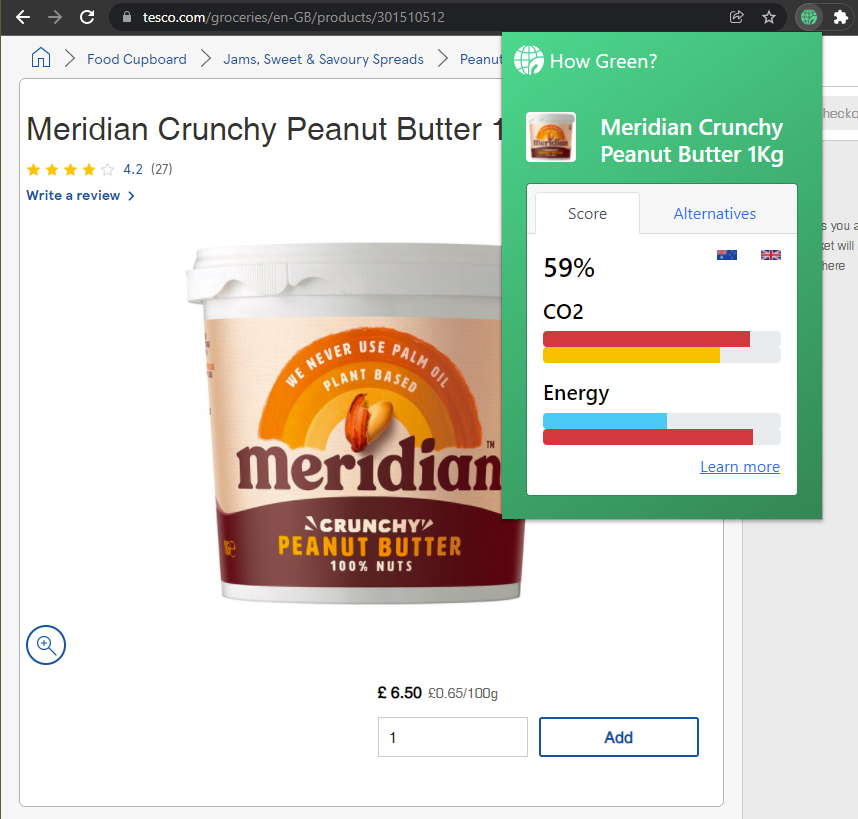
\includegraphics[width=0.9\columnwidth]{assets/final/product_page_with_score.png}
    \caption{Extension Displaying Product Score}
\end{figure}

Pressing the 'Learn More' button will lead the user to a more detailed review of the product on a new page rendered with Vue.js. At the bottom of the page are two buttons, 'View Graphs' and 'View Alternatives'. Clicking 'View Graphs' takes the user to the visualisations page, where the bar graph and radar graph are both displayed with Chart.js. The bar graph is used to compare the different metrics between products and the radar graph is used to view a side by side comparison of the current product's metrics and its alternatives' metrics.

\begin{figure}[h]
    \centering
    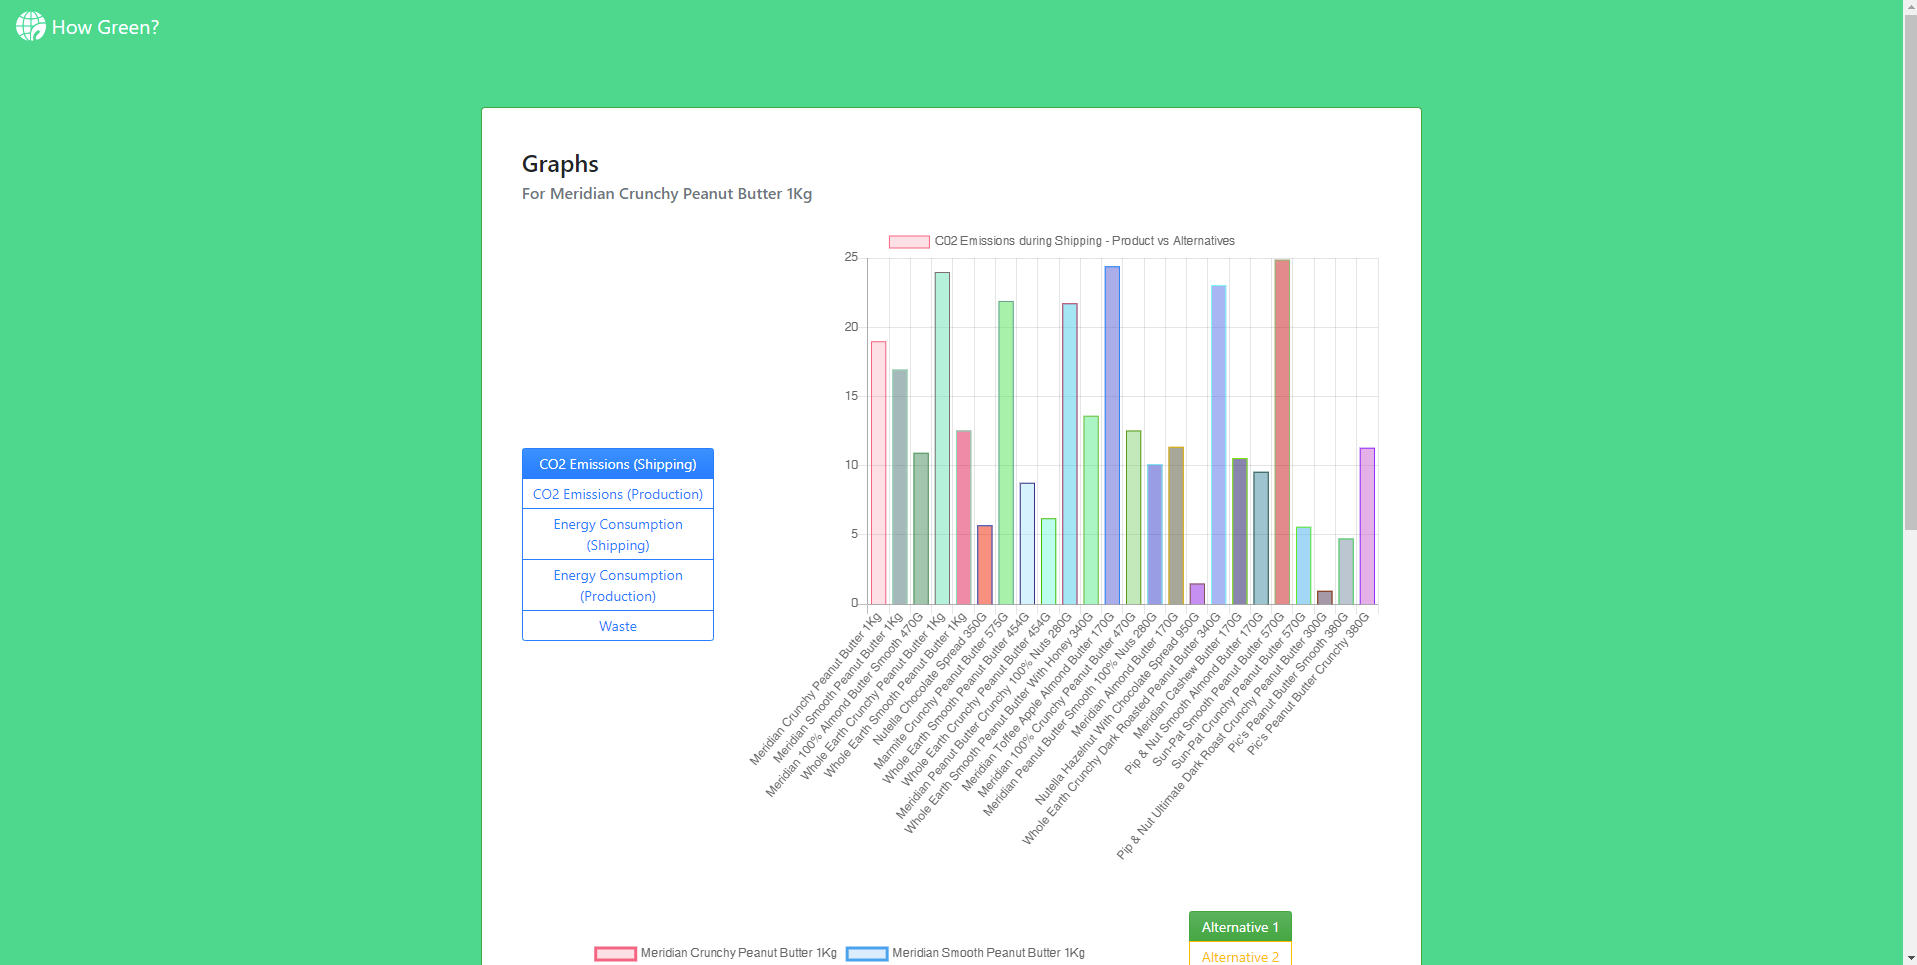
\includegraphics[width=0.9\columnwidth]{assets/final/visualisations_1.png}
    \caption{Bar graph visualisation}
\end{figure}

\begin{figure}[h]
    \centering
    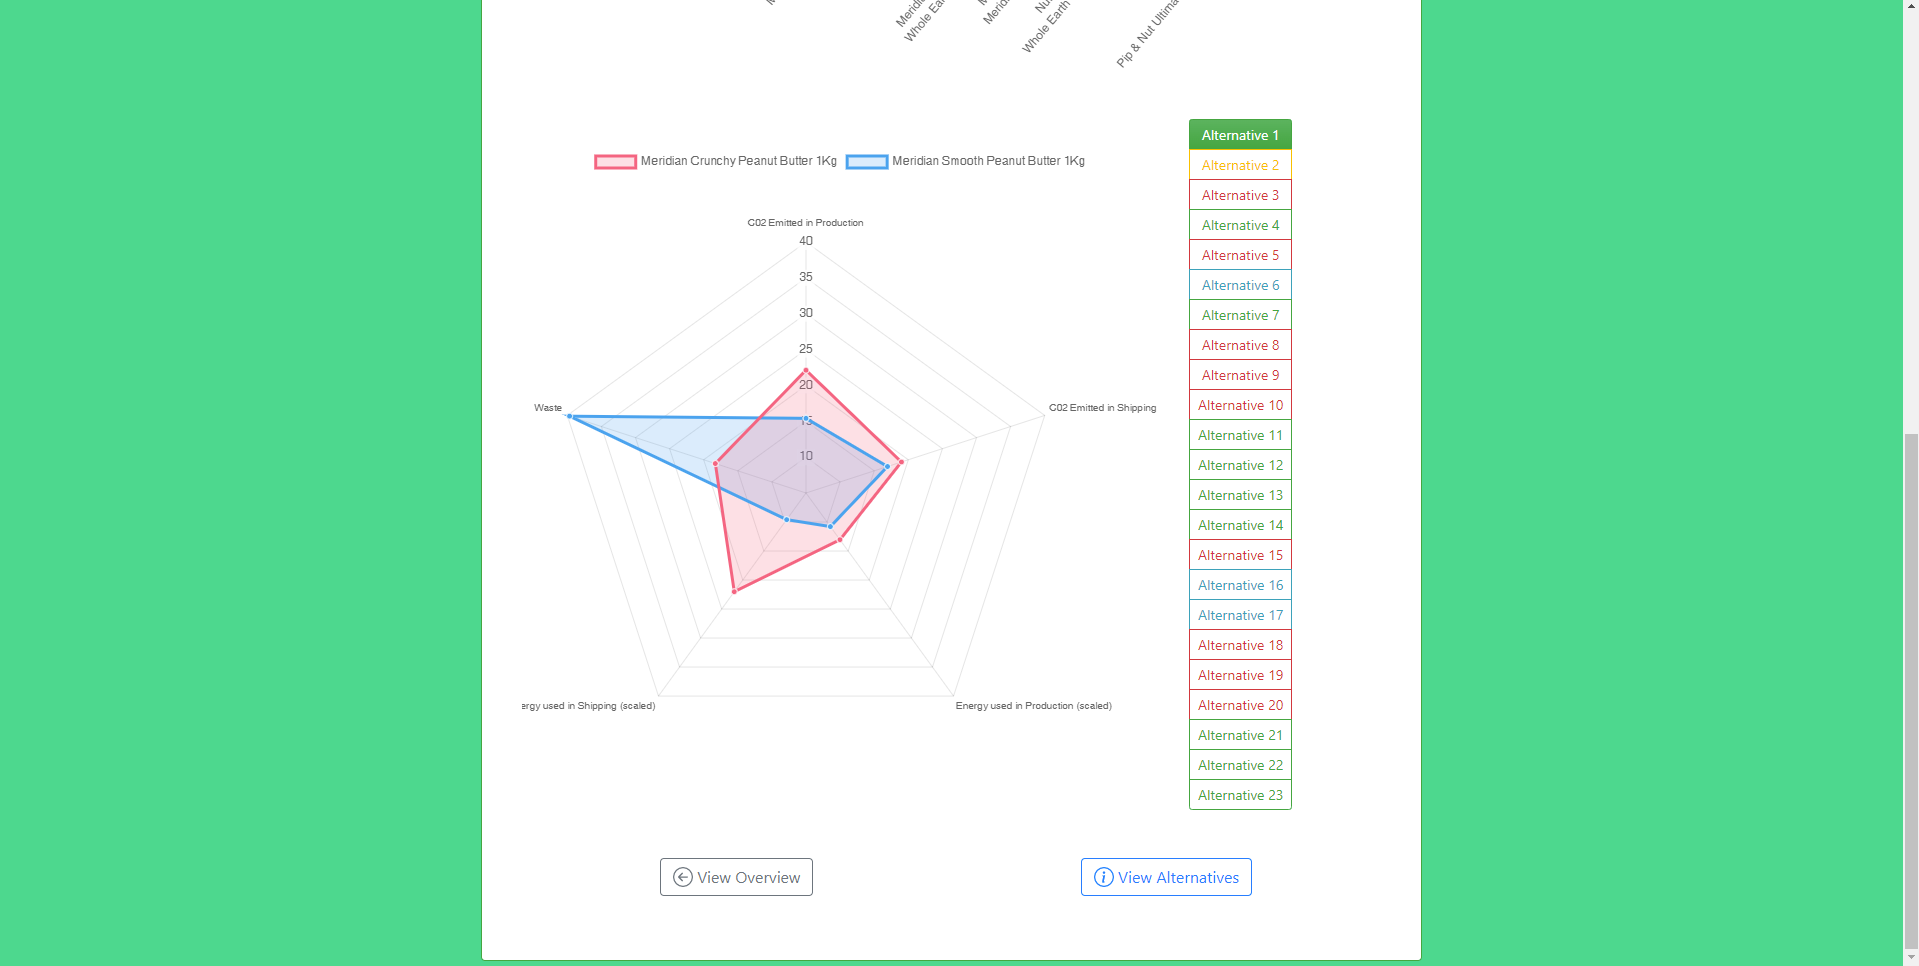
\includegraphics[width=0.9\columnwidth]{assets/final/visualisations_2.png}
    \caption{Radar graph visualisation}
\end{figure}

Clicking the 'View Alternatives' button will display a larger list of suggested alternatives of that product. The users from all of these pages have the option to go back to the How Green? home page or can go back to the Tesco's site by closing the window. 

\begin{figure}[h]
    \centering
    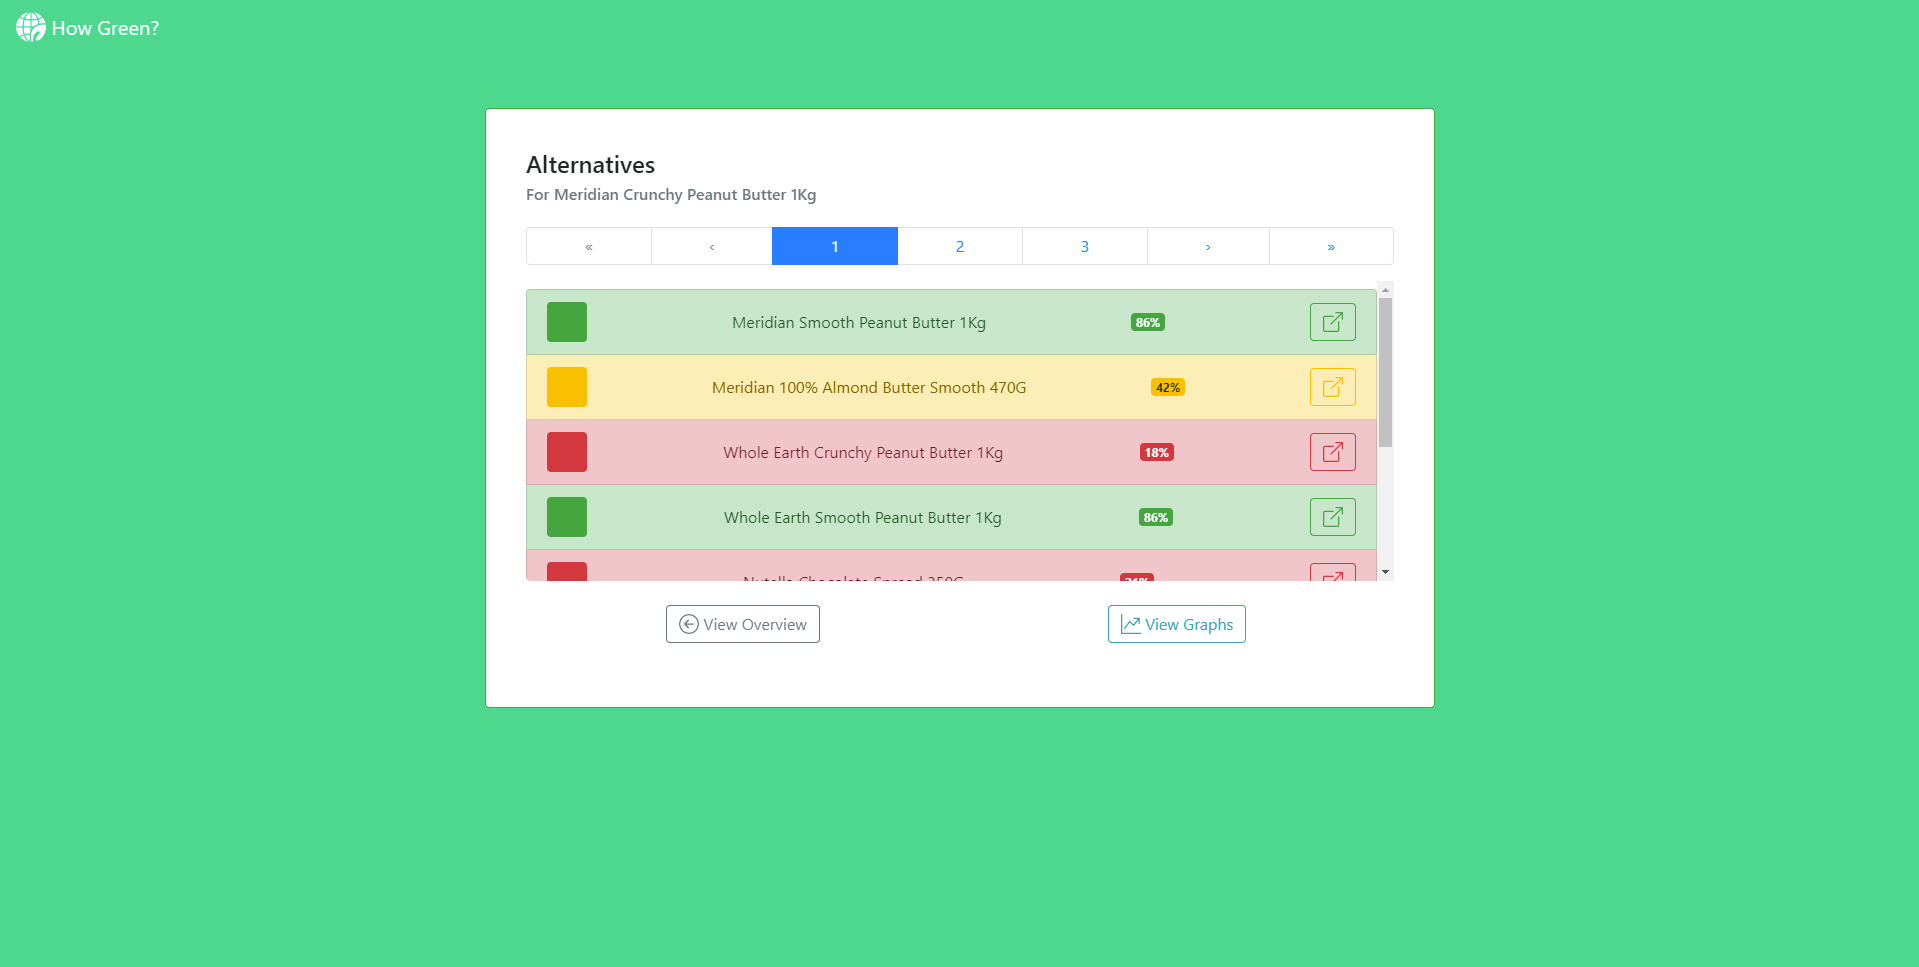
\includegraphics[width=0.9\columnwidth]{assets/final/product_alternatives_view_more.png}
    \caption{All alternative products}
\end{figure}

%==============================================================================
%% Evaluation

\section*{Final Evaluation}
% Summarize the results of the MVP think-aloud and survey results
With our MVP complete, we completed one final usability evaluation of our refined product. Given our small sample size, we decided to use a System Usability Survey (SUS) to measure the usability of our browser extension. The survey consists of 10 questions, each with 5 response options for respondents. Additionally, we followed up on the same survey questions administered after the Figma prototype, to ensure that our refined product was at least as good as, if not better than the Figma prototype.

The survey was administered after the completion of a think-aloud evaluation, following the same tasklist as used in the Figma prototype. This was again done intentionally to be able to compare our designs more directly. The evaluations were performed in a controlled setting, watched over by an evaluator to ensure a smooth procedure.

The results of the think-aloud evaluation will now be summarized , followed by a summary of the survey results as well as possible refinements to be made based on this evaluation:

\begin{itemize}
    \item In general, participants of the think-aloud evaluation noticed an improvement in overall design from the Figma prototype to the final version.
    \item However, participants also noted several issues with the final design which, if addressed, would improve the overall user experience.
    \item Participants mentioned that there should be some assistance when using the extension for the first time. For instance, waiting for the score to load after clicking the extension on a product page, felt confusing. The same participants agreed that most users would figure out how to use the extension quickly enough, but the uncertainty would be eliminated through a short tutorial. 
    \item The graphs page felt a little confusing to navigate towards the lower half. Participants referenced to the list of alternative buttons that act as switches for the second graph as a particular area of difficulty. 
    \item The graphs themselves also suffered from various information visualization issues, which should have been addressed in this final version. Specifically, the graphs need labels to be useful to users, since the information being displayed is only useful if the user can understand it. The score itself also needs an indication of what it means.
    \item In terms of quick visualizations, participants mentioned the traffic light system employed throughout the system was useful, however, the blue colour was confusing. 
    \item Finally, some participants noticed some additional features that would have made their experience more enjoyable. The search function on How Green's homepage supporting enter to search, was one such feature. This is understandable because enter to search is quite a standard convention for search systems.
\end{itemize}

Next we will provide a summary of the survey results:

\begin{itemize}
    \item The average score for the system usability survey was calculated, and found to be 83.8, corresponding with an excellent rating in terms of usability. All individual SUS scores (but one) scored higher than 68, deeming them all (but one) to be above average. This was particularly encouraging, given that though the final product still had numerous usability issues as addressed in the think-aloud evaluation, these issues clearly did not impact the overall usability of the system to a large extent.
    \begin{figure}[h]
        \centering
        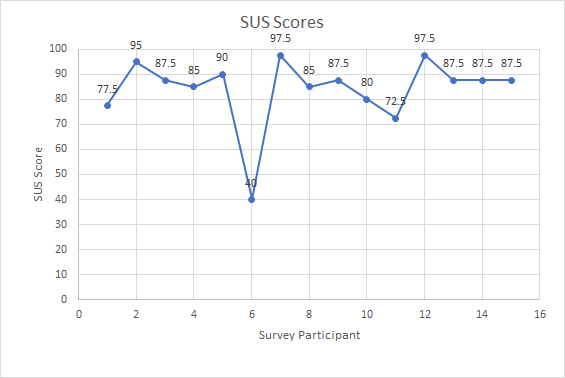
\includegraphics[width=0.9\columnwidth]{assets/final/SUS_distribution.jpg}
        \caption{SUS score distribution}
    \end{figure}
    \item Regarding the questions relating to the difficulty of performing each particular task, we again received positive survey results. All tasks but two (Tasks 4 \& 5), received lower ratings in difficulty in our final product when compared with the ratings from our Figma prototype. 
    \item The two tasks which users found more difficult to complete in our MVP, were finding the score for a product when on the product page, and showing further information from the browser extension. The inability to complete both these tasks was already addressed in our think-aloud evaluation results. This shows that the survey results correlate with our think-aloud results. Regarding the second task, specifically, there was an element of learning which made completing this task difficult in the final product. The Figma prototype had used a different method for completing this task, and many of the participants reflected this in attempting to complete the task in the same way.
\end{itemize}

Following from the results of our think-aloud evaluation and survey results, we identified numerous refinements to be applied to our product, had we had the time to implement these. These are summarised below:

\begin{itemize}
    \item Implement a short tutorial/guide for first time users, to run-through the entire system's navigation and features, once. Our reasoning here is that most participants felt comfortable using the system after being exposed to the entirety of it. 
    \item Improve the graphs used for information visualization. Specifically, add clear labelling, and explain any measurements used. 
    \item Add a clear indication of what the score means. \item Fix the traffic light system to be only red, yellow and green.
    \item Adhere to design conventions (enter for search).
\end{itemize}

%==============================================================================
%% Conclusion

\section*{Conclusions}
The How Green? MVP produced successfully meets the core requirements, helping users find more sustainable products based on the scores provided. How Green? allows users to see the score of products on the Tesco website while shopping by clicking on the Browser Extension. Users can view and interact with Information Visualisations on the product they were looking at and its alternatives.

Our development went through stages from a paper prototype onto a Figma prototype before How Green? was fully implemented. How Green? was implemented using Bootstrap React(TypeScript) for the Browser Extension. The application frontend was implemented using Vue, BootstapVue and Chart.js for the information visualisations. Finally, the application backend used web scraping by BeautifulSoup, and was implemented through a Flask(python) app.

An evaluation was carried out at all stages of the design process to give the team feedback and guidance in our refinements. Design ideas were evaluated initially by a focus group giving us a better idea of what users would expect from a sustainability based Browser Extension. This allowed us to focus on the area of online food shopping. The Figma prototype evaluation allowed us to identify what design users would like and how easy How Green? was to navigate through. The feedback sourced from these evaluations led to essential refinements that were addressed when implementing the final product. The final evaluation allowed us to see that users found How Green? usable and also outlined further areas for development.

With so many people using online shopping and an increased interest in sustainable shopping, if How Green? was to be completed and released we believe it would be a successful product.

\subsection*{Reflection}
Overall the final MVP we produced was successful, with users overall finding the Browser Extension easy to use and well designed. That being said, there are some areas that could be improved.

Having access to real data on products' real environmental impacts would actually allow users to be able to find out about the products they are buying. To further improve the app, purchasing access to data sources that provide information on products' environmental impact would be useful. Alternatively, further researching ways to calculate the environmental impact ourselves would be a worthy avenue to pursue. These would be feasible plans of action with a budget for the browser extension development or more development time.

Some features suggested in our initial focus group would have been nice to include if the extension was developed further. A warning system was suggested that would issue a warning that pops up to users when a product has a detrimental sustainability score. Implementing the browser extension popping up automatically was too complex for the time frame and could also be viewed as intrusive to users. Despite this, it is something that could possibly be implemented in the future if users would like this feature. Another feature mentioned by our initial focus group was the ability to sort and filter products based on price or popularity. This was another feature that that did not make our final implementation, but would likely be useful for users to have more control selecting products.

Our final evaluation produced feedback on the final implementation and provided us with some further refinements that could be implemented in the future. Users commented that the graphs were a little confusing with too many alternatives to compare. They also mentioned that the colour scheme used ended up being confusing. Both these issues could be addressed by reducing the number of alternative products and changing the underlying colour. A short tutorial was also recommended and would be useful to implement, making it easier for users to learn to use the system on the first try.

%==============================================================================
%% References & Appendix

\printbibliography

\section*{Appendix}

\begin{itemize}
    \item Our repository is available on GitHub at \url{https://github.com/ineshbose/how-green/}.
    \item Our paper prototype evaluation notes can seen on \url{https://docs.google.com/document/d/1Z9Yyng6E86i4iGeDRk46uSjJ6vv9AgSOIAffyQz66UQ/edit?usp=sharing}.
    \item Our interactive Figma prototype evaluation notes are available on \url{https://docs.google.com/document/d/1lc4_WFGwTevHNEQ-tcDoa3UE_lB9ZF0FNeryHLx6IW4/edit?usp=sharing}.
    \item Our interactive Figma prototype survey response summary is on \url{https://docs.google.com/forms/d/1R3aPlA1_waoi6QglShZzIZpRWmKeWJcedPadNIQyjS4/viewanalytics}.
    \item Our MVP evaluation notes are on \url{https://docs.google.com/document/d/1ofQff8n5nj1TBbIUzE1TqjlxPRCiPZxHQpxgCvUGYsc/edit?usp=sharing}.
    \item Our MVP survey response summary are available on \url{https://docs.google.com/forms/d/1TV6FeFKHaknJ9y61WBsk3vY-rAB2qxZyZFdMp_AxmPw/viewanalytics}.
    \item Our video demonstration and justification can be seen on \url{https://youtu.be/5TMIvUY2FYk}.
    \item The deployed homepage is hosted on \url{https://how-green.herokuapp.com/}.
\end{itemize}

\begin{figure}[h]
    \centering
    \includegraphics[width=0.9\columnwidth]{assets/appendix/Figma_home.PNG}
    \caption{How Green? Home page Figma}
\end{figure}

\begin{figure}[h]
    \centering
    \includegraphics[width=0.9\columnwidth]{assets/appendix/Figma_link.PNG}
    \caption{Figma Prototype links}
\end{figure}

\begin{figure}[h]
    \centering
    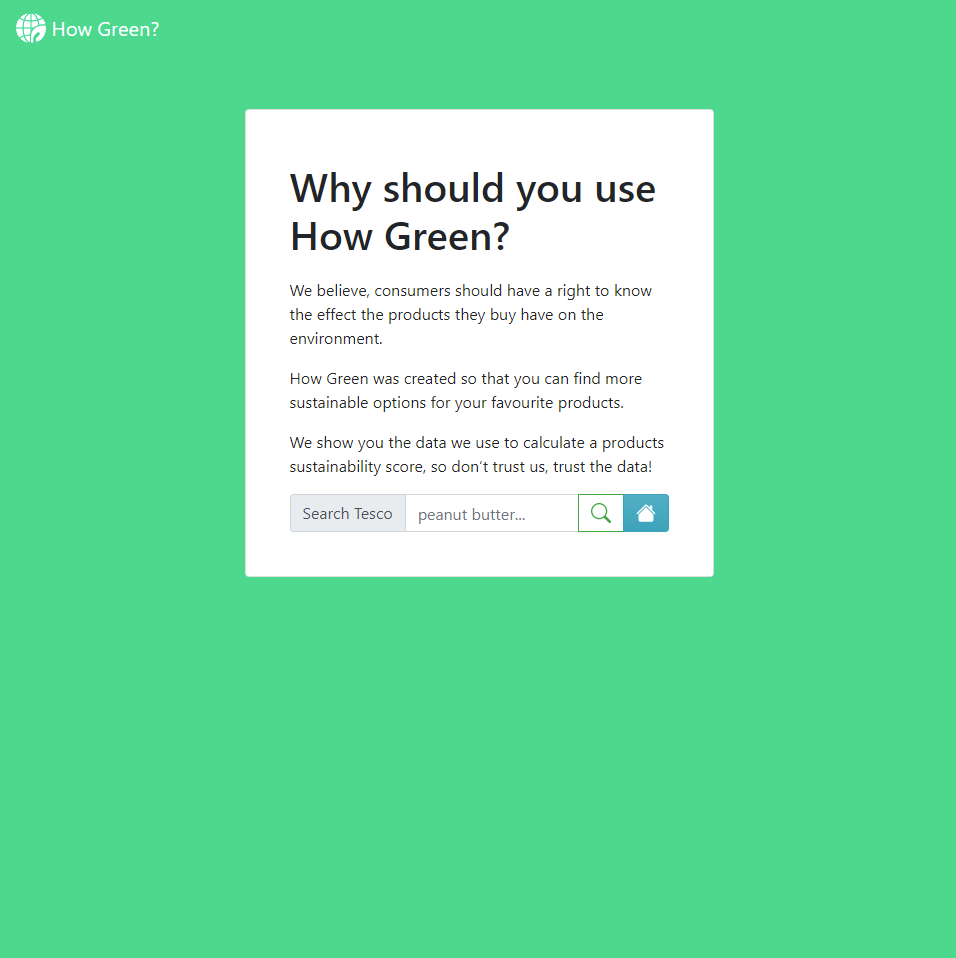
\includegraphics[width=0.9\columnwidth]{assets/final/landing_page.png}
    \caption{How Green Landing Page}
\end{figure}

\begin{figure}[h]
    \centering
    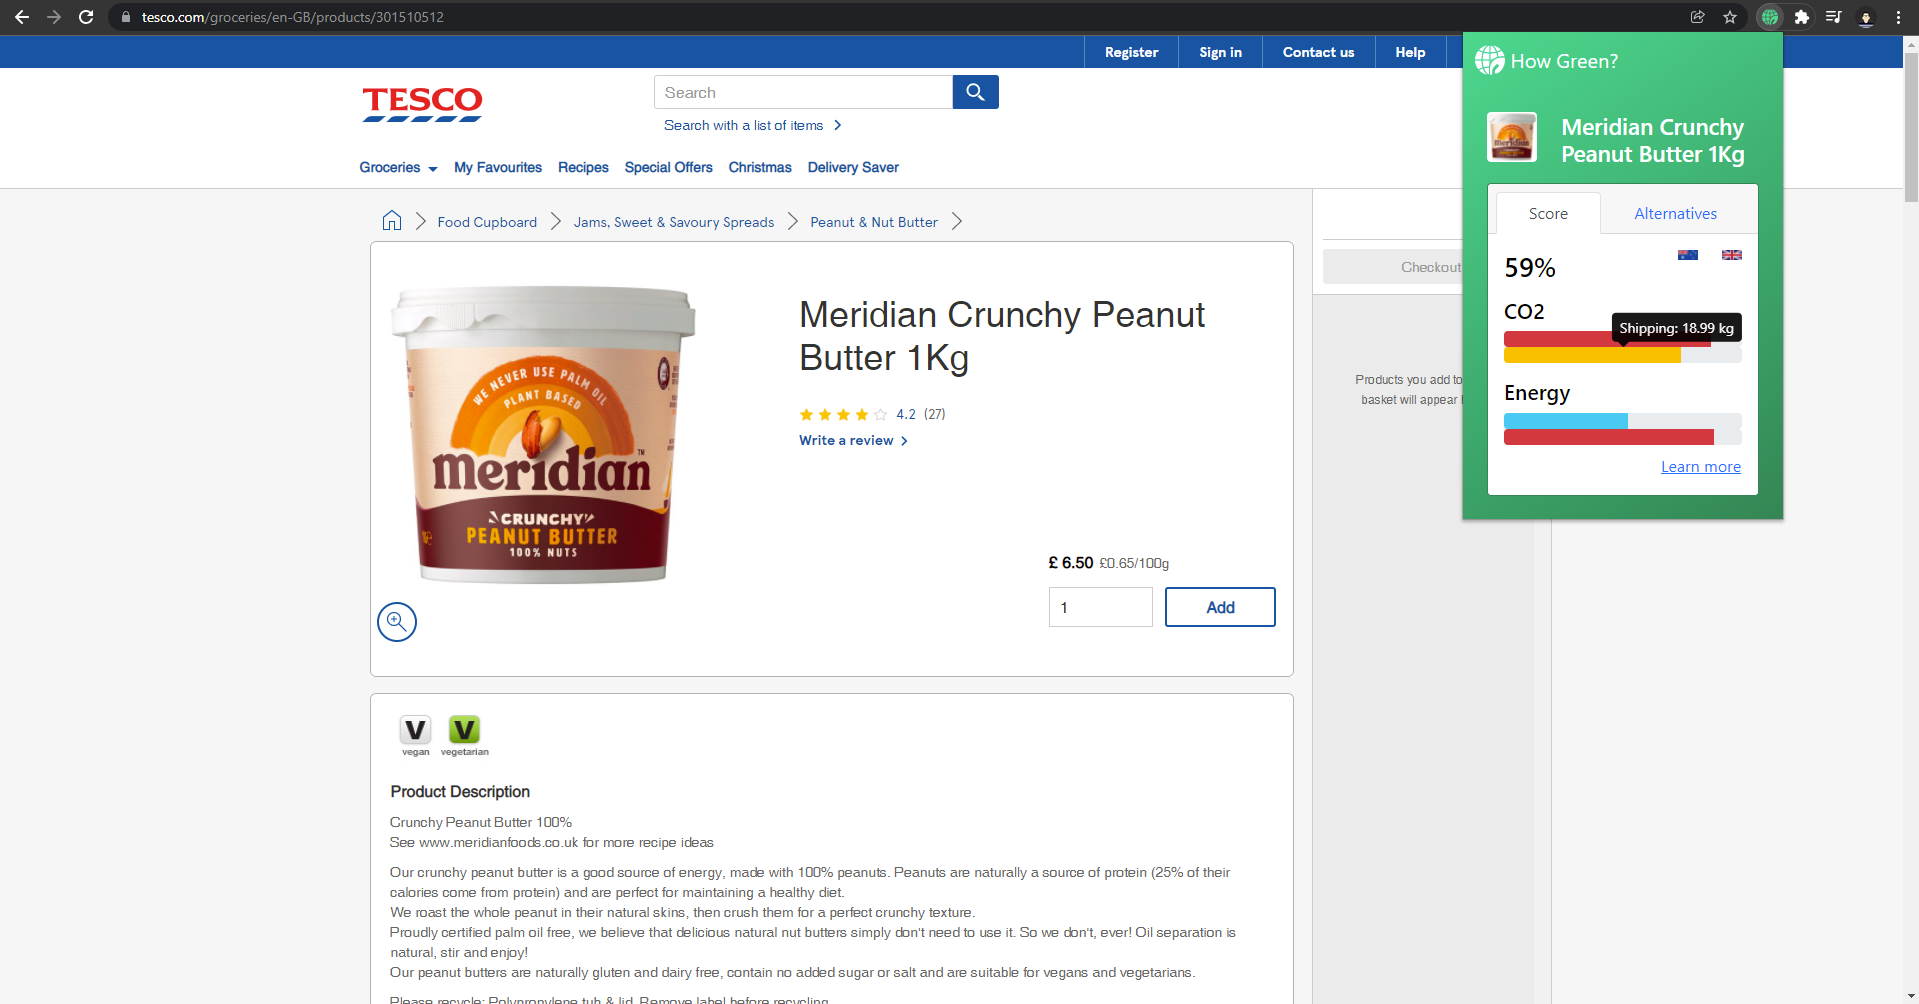
\includegraphics[width=0.9\columnwidth]{assets/final/extension_tooltips.png}
    \caption{How Green Browser Extension Tooltips}
\end{figure}

\begin{figure}[h]
    \centering
    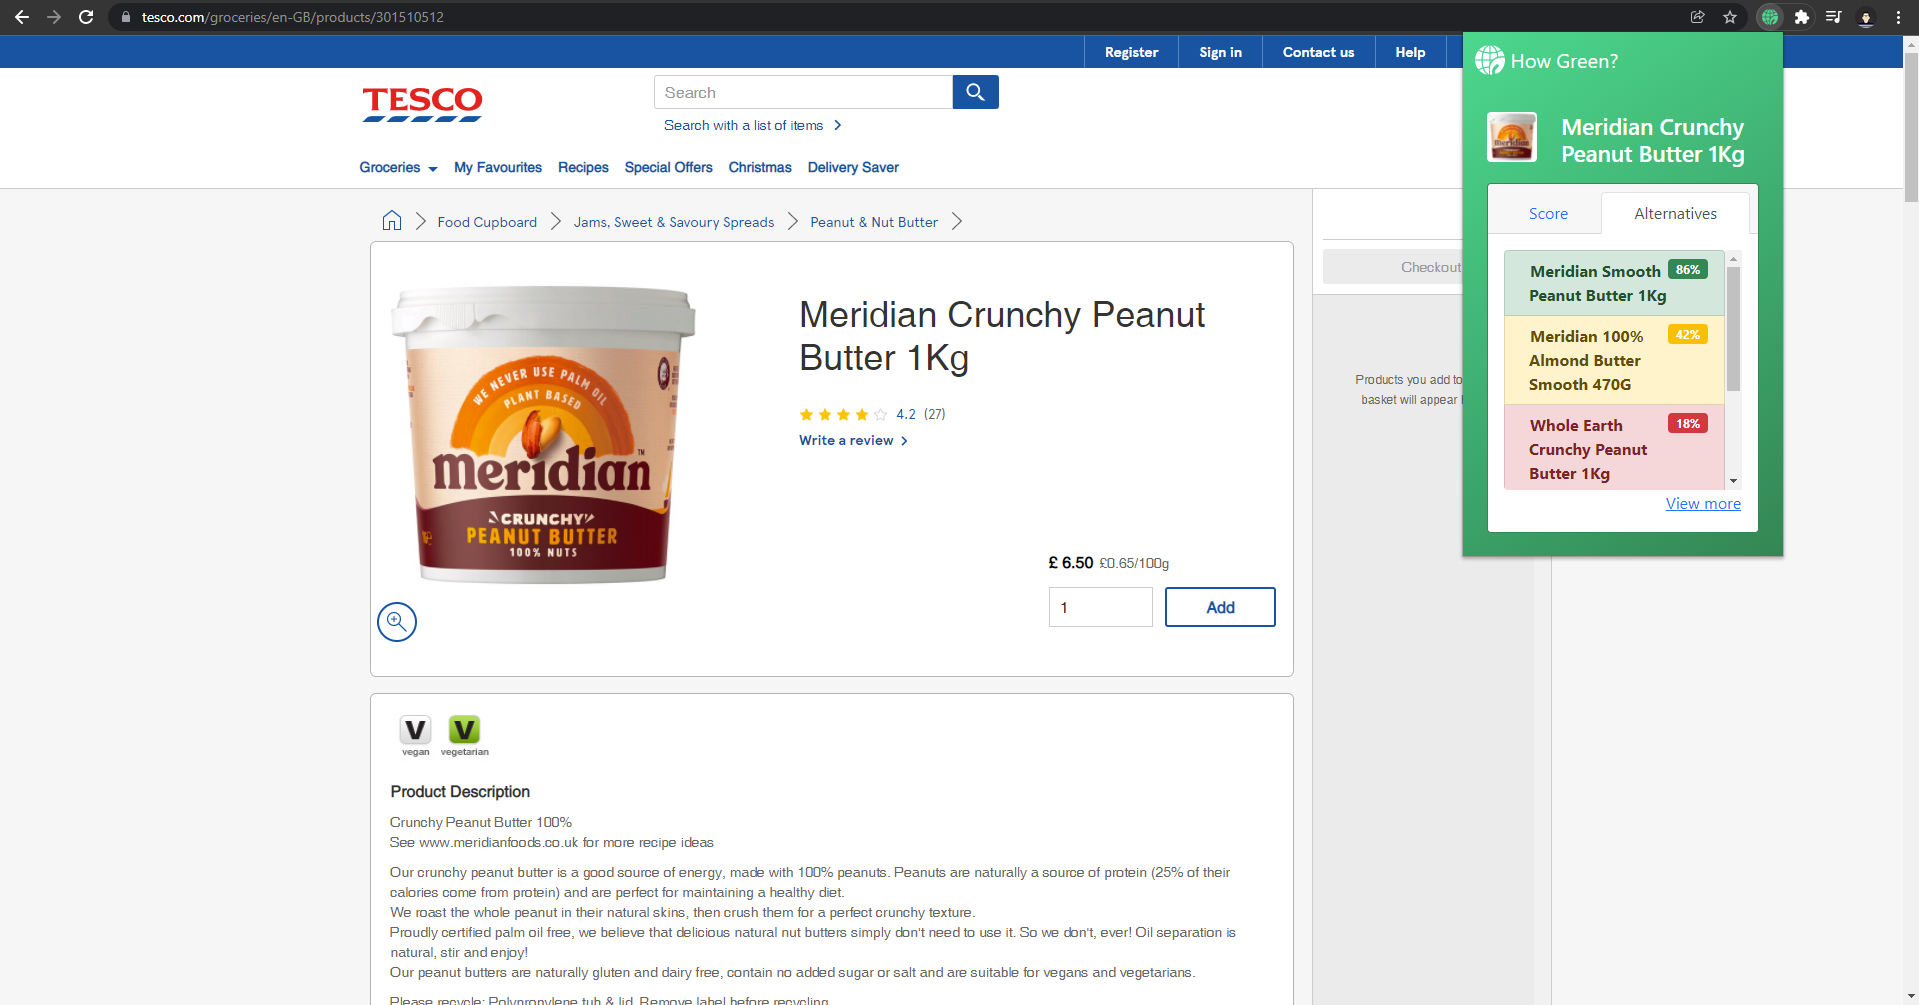
\includegraphics[width=0.9\columnwidth]{assets/final/product_page_with_alternatives.png}
    \caption{How Green Browser Extension Alternative Options}
\end{figure}

\begin{figure}[h]
    \centering
    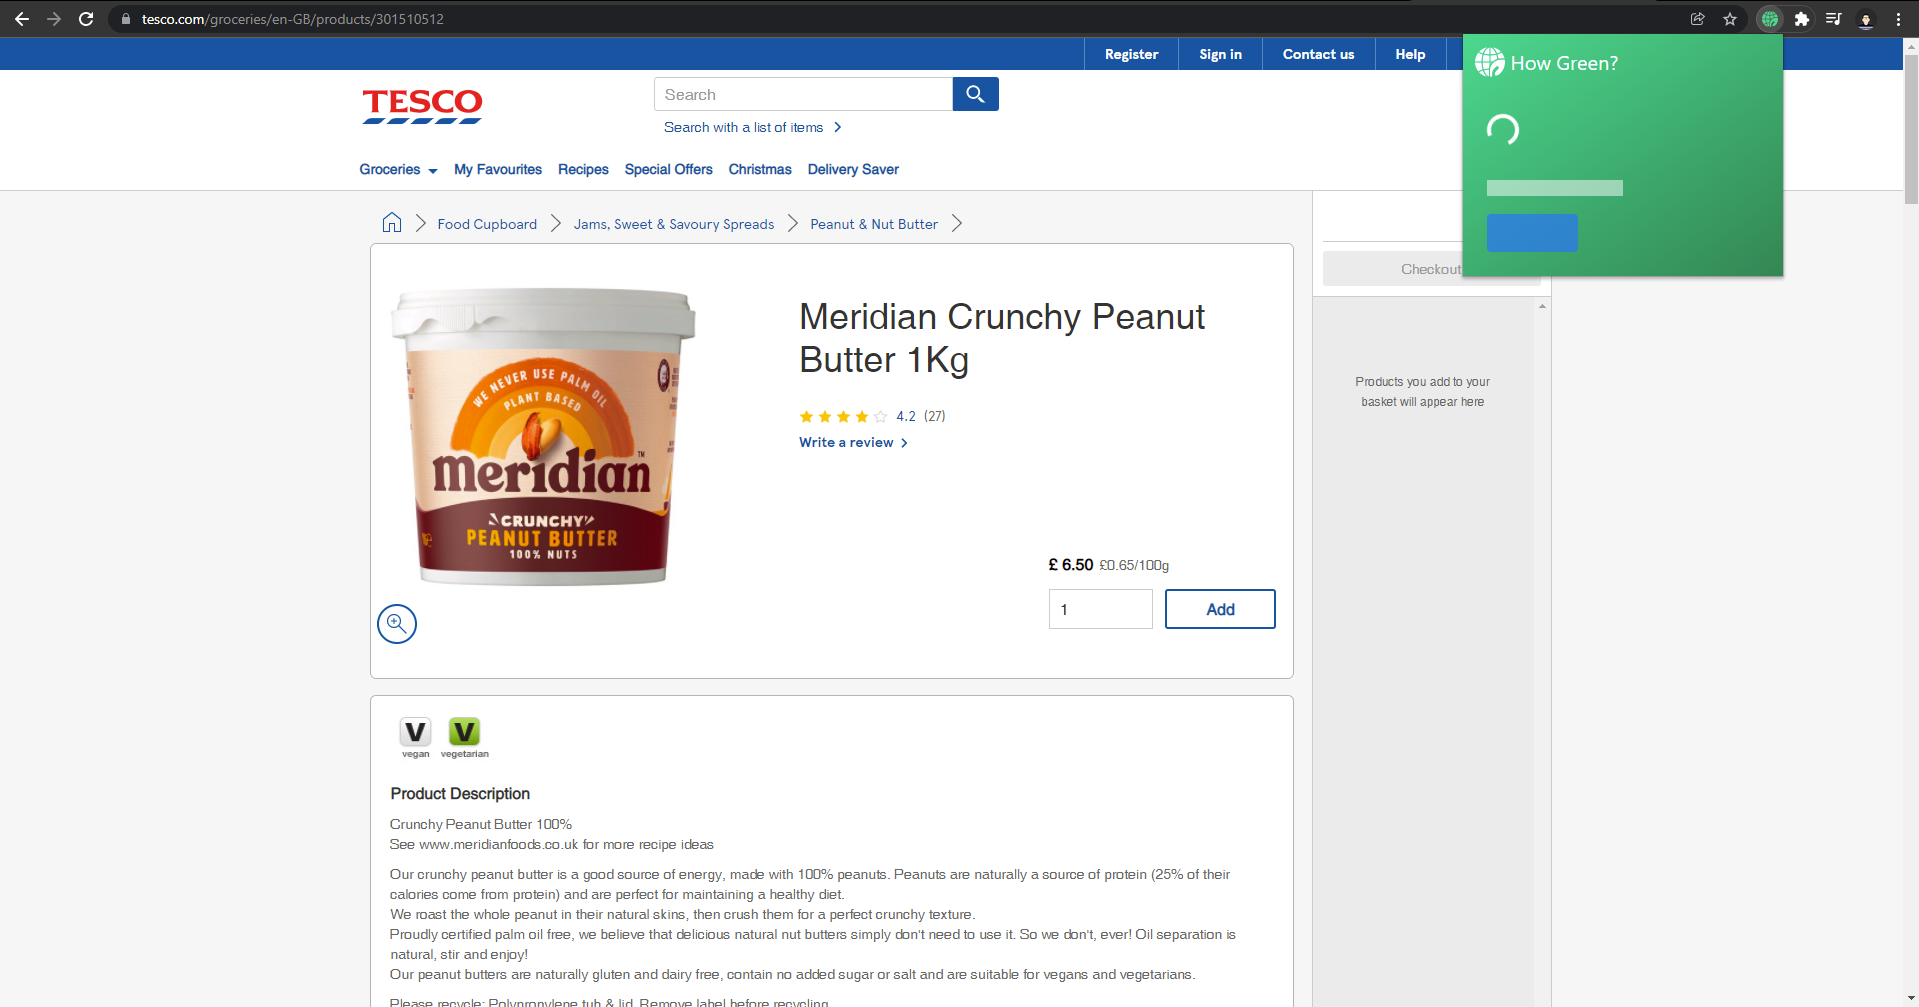
\includegraphics[width=0.9\columnwidth]{assets/final/extension_loading.png}
    \caption{How Green Browser Extension Loading}
\end{figure}


\begin{figure}[h]
\centering
\begin{minted}[bgcolor=bg]{text}
{
    "id": 301510512,
    "name": "Meridian Crunchy Peanut Butter...",
    "img": "...",
    "description": "...",
    "price": "£ 6.50",
    "score": 71,
    "origin": {
        "name": "Italy",
        "tld": "it"
    },
    "destination": {
        "name": "United Kingdom",
        "tld": "gb"
    },
    "distance": 2641,
    "fair_trade": false,
    "waste": 15.46,
    "co2": {
        "production": 7.14,
        "shipping": 10.22
    },
    "energy": {
        "production": 2147.12,
        "shipping": 9003.9
    },
    "alternatives": [
        {
            "id": "294224337",
            "name": "Whole Earth Crunchy...",
            "img": "...",
            "score": 49,
            "co2": { ... },
            "energy": { ... },
            "waste": 5.36
        },
        {
            ...
        },
        {
            "id": "263914432",
            "name": "Nutella Chocolate...",
            "img": "...",
            "score": 44,
            "co2": { ... },
            "energy": { ... },
            "waste": 20.35
        }
    ]
}
\end{minted}
\caption{Sample API response JSON data}
\end{figure}

\begin{center}
\end{center}

\end{document}
